\documentclass[a4paper,11pt]{report}

\usepackage[french]{babel}
\usepackage[utf8]{inputenc}
\usepackage[left=2.5cm,top=2cm,right=2.5cm,nohead,nofoot]{geometry}
\usepackage{url}
\usepackage{graphicx}
\usepackage{hyperref}
\usepackage{listings}
\usepackage{amsmath}
\usepackage{amssymb}
\usepackage{color}
\usepackage{listings}
\usepackage{float}
\DeclareMathOperator*{\join}{\bowtie}
\DeclareMathOperator*{\alpham}{\alpha}



\linespread{1.1}

\author{Bruno Rocha Pereira, Antoine Carpentier}
\title{Base de données : Villos}

\begin{document}

\lstset{
    breakatwhitespace=false,
    breaklines=true,
    escapeinside={\%*}{*},
    xleftmargin=5pt,
    xrightmargin=5pt,
    aboveskip=\bigskipamount,
    belowskip=\bigskipamount
}

\maketitle

\chapter{Introduction}

Le but de ce projet est de réaliser une application de gestion des Villos à Bruxelles en utilisant une base de données SQL et de traduire certaines requêtes en SQL, en algèbre relationnelle et en calcul relationnel tuple.
L'application doit permettre à différents types d'utilisateurs de s'inscrire, de se connecter et d'utiliser les Villos et à un administrateur de gérer les paiements qu'ils effectuent, d'effectuer des statistiques et de maintenir l'application.
Un programme permet d'importer les données fournies sous forme de fichiers CSV et XML dans une base de données SQL.
Le premier chapitre explique les choix effectués quant au langage de programmation, à la base de données et les modifications apportées au modèle de données fourni.
Le deuxième chapitre détaille le modèle de données à l'aide des diagrammes entités associations et relationnels.
Le troisième chapitre concerne les requêtes demandées en SQL, en algèbre relationnelle et en calcul relationnel tuple.

\chapter{Choix de conception}

\section{Langages}

Nous avons choisi \textbf{Python} car il contient un module de gestion pour \textbf{Sqlite3}. 
Nous avons également décidé d'utiliser \textbf{Flask}. Ce framework pour \textbf{Python}, associé au moteur de template \textbf{Jinja}, permet de générer facilement des pages HTML dynamiques. Pour compléter les pages HTML générées, nous avons rajouté du CSS pour les embellir et du Javascript pour pouvoir y ajouter une Google Map.

\section{Base de données}
Nous avons choisi \textbf{Sqlite3} comme gestionnaire de bases de données pour trois raisons. Tout d'abord, il permet de gérer des bases de données sans avoir besoin de serveur, en se basant simplement sur des fichiers. Ensuite, il est rapide et léger. Pour finir, \textbf{Python} gère nativement un accès a ces bases de données grâce au module \textbf{sqlite3}.
Le seul inconvénient est que \textbf{Sqlite3} ne possède pas beaucoup de fonctions natives mais il est extensible facilement en langage C.
Nous avons donc dû implémenter certaines fonctions mathématiques en C et les charger dans \textbf{Sqlite3}.

\chapter{Modèle et importation des données}

\section{Changements}
Nous avons légèrement modifié le modèle de données proposées dans les fichiers CSV et XML.
Premièrement, nous avons rajouté une entité \textbf{Administrateur} qui représente les administrateurs de l'application. Ceux-ci ont la possibilité d'effectuer des tâches de maintenance et de gestion telles que la visualisation des factures, la réparation des vélos, la visualisation des utilisateurs et de leurs voyages.
Deuxièmement, nous avons rajouté un attribut \textbf{Date de paiement} dans l'entité \textbf{Utilisateur Temporaire} qui permet de déterminer à l'aide de l'attribut \textbf{Date d'expiration} de la table \textbf{Utilisateur} la durée d'un ticket acheté par un utilisateur temporaire à des fins de facturation.
Troisièmement, nous avons rajouté une association à l'entité \textbf{Utilisateur} et à l'entité \textbf{Station} dans l'entité \textbf{Vélo} qui permet de faciliter les requêtes pour déterminer où se trouve un vélo, au prix d'une requête plus compliquée pour prendre un vélo et rendre un vélo.

\section{Modèle Entités-Associations}

\begin{figure}[H]
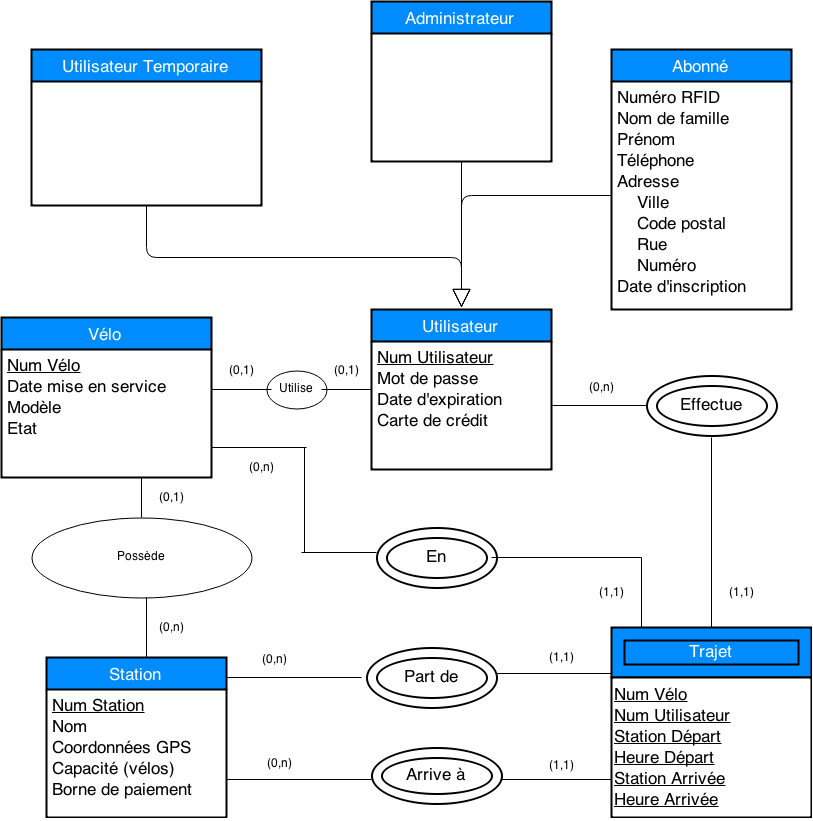
\includegraphics[scale=0.45]{MEA.png}
\centering
\caption{Modèle Entités-Associations}
\end{figure}

\subsection{Contraintes d'intégrités}
\begin{itemize}
\item Date mise en service d'un vélo plus petit que la date de départ d'un trajet avec ce vélo plus petit que date d'arrivée de ce trajet
\item Date d'expiration du compte utilisateur plus grand que la date d'inscription de ce compte
\item Date d'expiration du compte utilisateur plus grand que l'heure de départ d'un nouveau trajet de cet utilisateur
\item Deux abonnés ne peuvent pas avoir le même numéro RFID
\item Deux trajets ne peuvent pas utiliser le même vélo à la même période
\item Un vélo doit être en état de fonctionnement pour être utilisé dans un trajet
\item Le nombre de vélos dans une station donnée plus petit ou égal à la capacité de cette station
\item Deux stations différentes ne peuvent pas avoir les mêmes coordonnées GPS
\item Le nombre de vélos dans une station donnée plus grand ou égal à 0
\item Un utilisateur ne peut pas se connecter après la date d'expiration
\item Le nombre de vélos à la station de départ d'un trajet à l'heure du départ plus grand que 0
\item Le nombre de vélos à la station d'arrivée à l'heure d'arrivée plus petit que la capacité de cette station
\end{itemize}
\pagebreak
\section{Modèle Relationnel}

\textbf{Utilisateur} (\underline{NumUtilisateur}, MotDePasse, DateExpiration, CarteDeCredit)

\textbf{UtilisateurTemporaire} (\underline{NumUtilisateur})\\
  \phantom{Trajet}UtilisateurTemporaire.NumUtilisateur référence Utilisateur.NumUtilisateur

\textbf{Administrateur} (\underline{NumUtilisateur})\\
  \phantom{Trajet}Administrateur.NumUtilisateur référence Utilisateur.NumUtilisateur

\textbf{Abonné} (\underline{NumUtilisateur}, NumeroRFID, NomDeFamille, Prénom, Téléphone, AdresseVille,   AdresseCodePostal, AdresseRue, AdresseNumero, DateInscription)\\
  \phantom{Trajet}Abonné.NumUtilisateur référence Utilisateur.NumUtilisateur

\textbf{Vélo} (\underline{NumVelo}, DateMiseService, Modèle, Etat, Station, Utilisateur)\\
  \phantom{Trajet}Station référence Station.NumStation\\
  \phantom{Trajet}Utilisateur référence Utilisateur.NumUtilisateur

\textbf{Station} (\underline{NumStation}, Nom, CoordGPS, Capacité, BornePaiement)\\

\textbf{Trajet} (\underline{NumVelo, NumUtilisateur, StationDépart, HeureDépart, StationArrivée, HeureArrivée})\\
  \phantom{Trajet}NumVelo référence Vélo.NumVelo\\
  \phantom{Trajet}NumUtilisateur référence Utilisateur.NumUtilisateur\\
  \phantom{Trajet}StationDépart référence Station.NumStation\\
  \phantom{Trajet}StationArrivée référence Station.NumStation
  
  
\subsection{Contraintes d'intégrité}

\begin{itemize}
\item Pour tout Trajet, Trajet.HeureDépart doit être plus petit que Trajet.HeureArrivée.
\item Pour tout Trajet, Trajet.HeureDépart doit etre plus grand que Vélo.DateMiseEnService avec Trajet.NumVeo égal à Vélo.NumVelo
\item Il ne peut pas y avoir deux Trajet.NumUtilisateur identiques au même moment.
\item Il ne peut pas y avoir deux Trajet.NumVelo identiques au même moment.
\item Il ne peut pas y avoir deux Utilisateur.NumeroRFID identiques
\item Le nombre de Vélo.NumStation identiques à chaque Station.NumStation doit être plus petit que Station.Capacité
\item Il ne peut pas y avoir deux Station.CoordGPS identiques

\end{itemize}

\section{Programme d'importation des données}

Voici le script SQL de création de la base de données.

\lstinputlisting[language=sql]{../src/tables.sql}

Pour refléter les changements par rapport au modèle initial, le programme d'importation des données effectue trois tâches importantes.
Tout d'abord, il crée des \textbf{paymentDate} pour chaque \textbf{tempUsers} afin que la base de données soit cohérente. Les utilisateurs temporaires ainsi importés ont un ticket pour 7 jours.
Ensuite, à chaque insertion d'un enregistrement dans la table \textbf{trips}, il modifie les attributs \textbf{stationID} et \textbf{userID} de l'enregistrement correspondant dans la table \textbf{bicycles} afin de garder la trace de la position de chaque vélo.
Finalement, il crée un administrateur afin de pouvoir maintenir l'application.

\chapter{Requêtes}

\section{Requ\^ete 1}
    \begin{lstlisting}[language=sql]
    SELECT DISTINCT subs.userID, subs.lastname, subs.firstname, subs.addresscity, stations.name FROM trips 
    INNER JOIN subs ON subs.userID = trips.userID
    INNER JOIN stations ON trips.startStation = stations.stationID
    WHERE subs.addresscity='Ixelles' and stations.name = 'FLAGEY';
    \end{lstlisting}

    \begin{align}
    joinedTables \leftarrow trips \bowtie subs \bowtie_{startStation = stationID} \\
    filteredTables \leftarrow \sigma_{addresscity=Ixelles \bigwedge name=FLAGEY}(joinedTables)
    \end{align}

    \begin{align}
    \{ u.userID | subs(u) \wedge \exists t, trips(t) \wedge t.userID=u.userID \exists s, stations(s) \\
     \wedge t.startStation=s \wedge s.name=Flagey \wedge u.addresscity=Ixelles \}
    \end{align}

\section{Requ\^ete 2}
    \begin{lstlisting}[language=sql]
    SELECT DISTINCT trips2.userID
    FROM trips AS trips1
    INNER JOIN trips AS trips2 ON trips1.userID = trips2.userID AND trips1.startTime != trips2.startTime
    ORDER BY trips2.userID;

    \end{lstlisting}

    \begin{align}
    trips1 \leftarrow \alpha_{attributes:t1.attributes}(trips)\\
    trips2 \leftarrow \alpha_{attributes:t2.attributes}(trips)\\
    joinedTables \leftarrow trips1 \bowtie_{t1.userID=t2.userID \bigwedge t1.startTime != t2.startTime} trips2\\
    result \leftarrow \pi{t2.userID}
    \end{align}

    \begin{align}
    \{ u.userID | users(u) \wedge \exists t1, t2, trips(t1), trips(t2) \\
    \wedge t1.userID = t2.userID \wedge t1 != t2 \}
    \end{align}


\section{Requ\^ete 3}
    \begin{lstlisting}[language=sql]
    SELECT DISTINCT trip1.userID, trip2.userID
    FROM trips AS trip1
    INNER JOIN trips AS trip2 ON trip1.startStation = trip2.startStation AND trip1.endingStation = trip2.endingStation AND trip1.userID != trip2.userID;
    \end{lstlisting}

    \begin{align}
    trips1 \leftarrow \alpha_{attributes:t1.attributes}(trips)\\
    trips2 \leftarrow \alpha_{attributes:t2.attributes}(trips)\\
    joinedTables \leftarrow trips1 \bowtie_{t1.startStation = t2.startStation
    \bigwedge t1.endingStation = t2.endingStation \bigwedge t1.userID != t2.userID } trips2 \\
    result \leftarrow \pi_{t1.userID,t2.userID}(joinedTables)
    \end{align}

    \begin{align}
    \{u1.userID, u2.userID | users(u1), users(u2) \\
    \wedge \exists t1, t2, trips(t1), trips(t2) \\
    \wedge t1.userID=u1.userID \wedge t2.userID=u2.userID \\
    \wedge t1.startStation = t2.startStation \\
    \wedge t1.endingStation = t2.endingStation\}
    \end{align}


\section{Requ\^ete 4}
    \begin{lstlisting}[language=sql]
    SELECT DISTINCT trip1.endingStation, trip1.endingTime, trip2.startStation, trip2.startTime
    FROM trips AS trip1
    INNER JOIN trips AS trip2 ON trip1.bicycleID = trip2.bicycleID AND trip1.startTime < trip2.startTime
    GROUP BY trip2.startTime
    HAVING trip1.endingStation != trip2.startStation
    ORDER BY trip1.startTime ASC
    \end{lstlisting}
    \begin{align}
    trips1 \leftarrow \alpha_{attributes:t1.attributes}(trips)\\
    trips2 \leftarrow \alpha_{attributes:t2.attributes}(trips)\\
    joinedTables \leftarrow trips1 \bowtie_{t1.bicycleID = t2.bicycleID \bigwedge t1.startTime < t2.startTime} trips2 \\
    filteredTables \leftarrow \sigma_{t1.endingStation != t2.startStation} (\gamma_{t2.startTime}(joinedTables))\\
    result \leftarrow \pi t1.endingStation, t1.endingTime, t2.startStation, t2.startTime
    \end{align}

    \begin{align}
    \{ b.bicycleID | bicycles(b) \wedge \exists t1, t2, trips(t1), trips(t2) \\
    \wedge t1.bicycleID = b.bicycleID \wedge t2.bicycleID = b.bicycleID \\
    \wedge t2.startTime > t1.startTime \wedge \nexists t3, trips(t3) \\
    \wedge t3.startTime > t1.endingTime \wedge t3.endingTime < t2.startTime \\
    \wedge t1.endingStation != t2.startStation \}
    \end{align}


\section{Requ\^ete 5}
    \begin{lstlisting}[language=sql]
    SELECT users.userID, subs.lastname, subs.firstname,
        (CASE WHEN subs.subscribeDate IS NOT NULL THEN subs.subscribeDate ELSE tempUsers.paymentDate END) AS subscribeDate,
        COUNT(*) AS total_trips,
        SUM(sqrt(power((s1.coordX-s2.coordX)*71, 2) + power((s1.coordY-s2.coordY)*111, 2))) AS total_distance
    FROM trips
    INNER JOIN users ON users.userID = trips.userID
    INNER JOIN stations AS s1 ON s1.stationID = trips.startStation
    INNER JOIN stations AS s2 ON s2.stationID = trips.endingStation
    LEFT OUTER JOIN subs ON subs.userID = users.userID
    LEFT OUTER JOIN tempUsers ON tempUsers.userID = users.userID
    GROUP BY trips.userID
    HAVING total_distance/total_trips
    ORDER BY COUNT(trips.userID);
    \end{lstlisting}


\section{Requ\^ete 6}
    \begin{lstlisting}[language=sql]
    SELECT stations.name, COUNT(trips.endingStation), COUNT(DISTINCT trips.userID)
    FROM stations
    INNER JOIN trips ON trips.endingStation = stations.stationID
    GROUP BY trips.endingStation
    HAVING COUNT(trips.endingStation) >= 10;
    \end{lstlisting}

\chapter{Requ\^etes additionnelles}

    \section{Billing}
    \begin{lstlisting}[language=sql]
    SELECT COUNT(*) 
    FROM users
    INNER JOIN subs ON subs.userID = users.userID
    WHERE subs.subscribeDate <= ?
    AND (strftime('%m/%Y', users.expiryDate) = ? OR strftime('%Y', users.expiryDate) = ?) 
        OR strftime('%m/%Y', subs.subscribeDate) = ? OR strftime('%Y', subs.subscribeDate) = ?
    \end{lstlisting}

    \begin{lstlisting}[language=sql]

    SELECT COUNT(*)
    FROM tempUsers
    INNER JOIN users ON tempUsers.userID = users.userID
    WHERE users.expiryDate >= ? AND users.expiryDate <= ?
    AND CAST((julianday(users.expiryDate) - julianday(tempUsers.paymentDate)) AS INTEGER) == ?
    \end{lstlisting}

    \begin{lstlisting}[language=sql]

    SELECT
        SUM(CASE 
            WHEN duration = 1 THEN 0 
            WHEN duration = 2 THEN 0.5 
            WHEN duration = 3 THEN 1.5 
            ELSE (duration-3) * 2 + 1.5 
        END)
    FROM 
    (SELECT CAST((CEIL((julianday(endingTime) - julianday(startTime)) * 48.0)) AS INTEGER) AS duration
    FROM trips
    WHERE startTime >= ? AND startTime <= ? AND endingStation IS NOT NULL AND endingTime IS NOT NULL)
    \end{lstlisting}



\end{document}